\documentclass[floatsintext,man]{apa6}

\usepackage{amssymb,amsmath}
\usepackage{ifxetex,ifluatex}
\usepackage{fixltx2e} % provides \textsubscript
\ifnum 0\ifxetex 1\fi\ifluatex 1\fi=0 % if pdftex
  \usepackage[T1]{fontenc}
  \usepackage[utf8]{inputenc}
\else % if luatex or xelatex
  \ifxetex
    \usepackage{mathspec}
    \usepackage{xltxtra,xunicode}
  \else
    \usepackage{fontspec}
  \fi
  \defaultfontfeatures{Mapping=tex-text,Scale=MatchLowercase}
  \newcommand{\euro}{€}
\fi
% use upquote if available, for straight quotes in verbatim environments
\IfFileExists{upquote.sty}{\usepackage{upquote}}{}
% use microtype if available
\IfFileExists{microtype.sty}{\usepackage{microtype}}{}

% Table formatting
\usepackage{longtable, booktabs}
\usepackage{lscape}
% \usepackage[counterclockwise]{rotating}   % Landscape page setup for large tables
\usepackage{multirow}		% Table styling
\usepackage{tabularx}		% Control Column width
\usepackage[flushleft]{threeparttable}	% Allows for three part tables with a specified notes section
\usepackage{threeparttablex}            % Lets threeparttable work with longtable

% Create new environments so endfloat can handle them
% \newenvironment{ltable}
%   {\begin{landscape}\begin{center}\begin{threeparttable}}
%   {\end{threeparttable}\end{center}\end{landscape}}

\newenvironment{lltable}
  {\begin{landscape}\begin{center}\begin{ThreePartTable}}
  {\end{ThreePartTable}\end{center}\end{landscape}}




% The following enables adjusting longtable caption width to table width
% Solution found at http://golatex.de/longtable-mit-caption-so-breit-wie-die-tabelle-t15767.html
\makeatletter
\newcommand\LastLTentrywidth{1em}
\newlength\longtablewidth
\setlength{\longtablewidth}{1in}
\newcommand\getlongtablewidth{%
 \begingroup
  \ifcsname LT@\roman{LT@tables}\endcsname
  \global\longtablewidth=0pt
  \renewcommand\LT@entry[2]{\global\advance\longtablewidth by ##2\relax\gdef\LastLTentrywidth{##2}}%
  \@nameuse{LT@\roman{LT@tables}}%
  \fi
\endgroup}


  \usepackage{graphicx}
  \makeatletter
  \def\maxwidth{\ifdim\Gin@nat@width>\linewidth\linewidth\else\Gin@nat@width\fi}
  \def\maxheight{\ifdim\Gin@nat@height>\textheight\textheight\else\Gin@nat@height\fi}
  \makeatother
  % Scale images if necessary, so that they will not overflow the page
  % margins by default, and it is still possible to overwrite the defaults
  % using explicit options in \includegraphics[width, height, ...]{}
  \setkeys{Gin}{width=\maxwidth,height=\maxheight,keepaspectratio}
\ifxetex
  \usepackage[setpagesize=false, % page size defined by xetex
              unicode=false, % unicode breaks when used with xetex
              xetex]{hyperref}
\else
  \usepackage[unicode=true]{hyperref}
\fi
\hypersetup{breaklinks=true,
            pdfauthor={},
            pdftitle={The Development of Color Terms in Shipibo-Konibo Children},
            colorlinks=true,
            citecolor=blue,
            urlcolor=blue,
            linkcolor=black,
            pdfborder={0 0 0}}
\urlstyle{same}  % don't use monospace font for urls

\setlength{\parindent}{0pt}
%\setlength{\parskip}{0pt plus 0pt minus 0pt}

\setlength{\emergencystretch}{3em}  % prevent overfull lines


% Manuscript styling
\captionsetup{font=singlespacing,justification=justified}
\usepackage{csquotes}
\usepackage{upgreek}

 % Line numbering
  \usepackage{lineno}
  \linenumbers


\usepackage{tikz} % Variable definition to generate author note

% fix for \tightlist problem in pandoc 1.14
\providecommand{\tightlist}{%
  \setlength{\itemsep}{0pt}\setlength{\parskip}{0pt}}

% Essential manuscript parts
  \title{The Development of Color Terms in Shipibo-Konibo Children}

  \shorttitle{Color Terms in Shipibo-Konibo Children}


  \author{Danielle Kellier*\textsuperscript{1}, Martin Fortier*\textsuperscript{2}, Maria Fernández Flecha\textsuperscript{3}, \& Michael C. Frank\textsuperscript{4}}

  % \def\affdep{{"", "", "", ""}}%
  % \def\affcity{{"", "", "", ""}}%

  \affiliation{
    \vspace{0.5cm}
          \textsuperscript{1} University of Pennsylvania\\
          \textsuperscript{2} PSL Research University\\
          \textsuperscript{3} Pontificia Universidad Católica del Perú\\
          \textsuperscript{4} Stanford University  }

  \authornote{
    * these authors contributed equally.
    
    MCF was supported by a Jacobs Foundation Fellowship. We are especially
    grateful to Paul Kay for assistance throughout the study.
    
    Correspondence concerning this article should be addressed to Martin
    Fortier*, Postal address. E-mail:
    \href{mailto:martin.fortier@ens.fr}{\nolinkurl{martin.fortier@ens.fr}}
  }


  \abstract{Enter abstract here. Each new line herein must be indented, like this
line.}
  \keywords{keywords \\

    \indent Word count: X
  }





\usepackage{amsthm}
\newtheorem{theorem}{Theorem}[section]
\newtheorem{lemma}{Lemma}[section]
\theoremstyle{definition}
\newtheorem{definition}{Definition}[section]
\newtheorem{corollary}{Corollary}[section]
\newtheorem{proposition}{Proposition}[section]
\theoremstyle{definition}
\newtheorem{example}{Example}[section]
\theoremstyle{definition}
\newtheorem{exercise}{Exercise}[section]
\theoremstyle{remark}
\newtheorem*{remark}{Remark}
\newtheorem*{solution}{Solution}
\begin{document}

\maketitle

\setcounter{secnumdepth}{0}



TO BE PASTED FROM GOOGLE DOC

\section{Experiment 1}\label{experiment-1}

In our first experiment, our goal was to replicate and update the
characterization of the adult SK color system given by the World Color
Survey. We were further interested in the use of Spanish terms as
language contact and multilingualism have increased in the years since
the original World Color Survey work.

\subsection{Methods}\label{methods}

\subsubsection{Participants}\label{participants}

We recruited 39 adult participants (7 men). Most of participants were
from SK communities of the Middle Ucayali region (from Yarinacocha, San
Francisco, and Nueva Betania), but some of them were from communities of
the Lower (Paoyhan) and Upper (Puerto Belen) Ucayali. In Yarinacocha (a
small town located in the vicinity of Pucallpa), participants were
recruited in Bena Jema, a neighborhood where most of the inhabitants are
SK. All the other places where participants were recruited were native
community villages exclusively inhabited by SK people. Overall, the
sample included both somewhat urbanized SK (Yarinacocha and San
Francisco) as well as SK individuals who were still used to more
traditional activities and regular contact with the surrounding
rainforest (Nueva Betania, Paoyhan, and Puerto Belen).

The median self-reported age for participants was 38 years with a range
between 20 to 64 years of age (SD = 13.60yo). Regarding occupations,
41\% of the women were homemakers (33\% overall) and another 41\% were
artisans (33\%). Three of the 7 men were horticulturalists (43\%, 8\%
overall). Four women (12\%, 10\% overall) and three men (43\%, 8\%
overall) identified as students.

Although all adult participants spoke Shipibo-Konibo as a first
language, all were bilingual to a substantial degree. All reported an
introduction to the Spanish language before early adolescence (\emph{M}
= 7.80yo, \emph{SD} = 2.90y). Participant age and reported age of
introduction to Spanish were positively correlated; younger participants
reported learning Spanish at an early age although all participants
reported introductions before early adolescence (\emph{r} = 0.43,
\emph{p} = 0.01).

\subsection{Materials}\label{materials}

We used the 330 Munsell color chips as stimuli for the study. However,
only 165 chips were used for each single participant (see below). These
chips were exactly those used to collect data for the WCS. Individual
color chips were 2 cm x 2.5 cm.

\subsection{Procedure}\label{procedure}

In order to make sure that the natural light intensity would not vary
much between participants, the experiment took place indoors, near a
window or a door. The study was conducted entirely in the SK language.

Our procedure was similar to that used in the WCS (see Kay, Berlin,
Maffin, Merrifield, \& Cook, 2009, pp. 585--591). Participants were
seated in front of the experimenter and introduced to the whole
procedure and the general goal of the study. Then the primary procedure
involved presenting participants with a color chip and asking them:
\enquote{What is the color of this chip?}\footnote{The SK word for color
  that we used was the Spanish word \emph{color}. In general, the SK
  language includes some castillanisms that are well-known by all
  speakers; color is one of them.} and recording their response or
responses.

One major difference between the WCS procedure and ours is that, in the
WCS, the experimenter was expected to brief participants so that they
would only provide basic color terms during the task (e.g.,
\enquote{blue} as opposed to \enquote{navy blue} or \enquote{sky-like}).
However, we found it rather difficult to help participants understand in
a few sentences what a basic color term was.\footnote{Indeed, as Berlin
  \& Kay (2009: 587-589) acknowledge, there is no straightforward
  necessary and sufficient criteria for the \enquote{basicness} of a
  color term.} Thus, we opted to let participants provide any term they
wished. If they did not provide a basic color term, we would ask further
questions to elicit a basic color term. For example, if the participant
provided the term \enquote{blood-like} (a non-basic color term) when
presented with a red color chip, the experimenter would ask: \enquote{Do
you know of any other word to refer to the color of this chip?} If the
participant subsequently responded \enquote{dark red} (another non-basic
color term), the experimenter would further ask: \enquote{How would you
refer to this color with only one word?} Eventually, the participant
would say \enquote{red} (a basic color term).

For some chips, participants would provide a basic color term at once;
but for others, they would first provide one or two non-basic terms
before actually providing a basic term. When participants did not
provide a basic color term after three trials (i.e., two follow-up
questions), no further questions was asked, and the experimenter
proceeded to the next chip. This method was more effortful and
time-consuming than the WCS procedure, but it improved the fluency and
the intuitiveness of the task for participants.

A second difference between our procedure and that of the WCS concerned
the number of chips each participant was presented with. In the WCS,
every participant was expected to provide color terms for each of the
330 chips of the set. As we were afraid that doing so would take too
long and that participants would find the task tedious, we decided that
the set of chips would be split in two (even and uneven numbers) and
that every participant would be randomly ascribed to one of the two
subsets. As a result, each participant was presented with only 165
chips.

\subsection{Results and Discussion}\label{results-and-discussion}

\begin{figure}
\centering
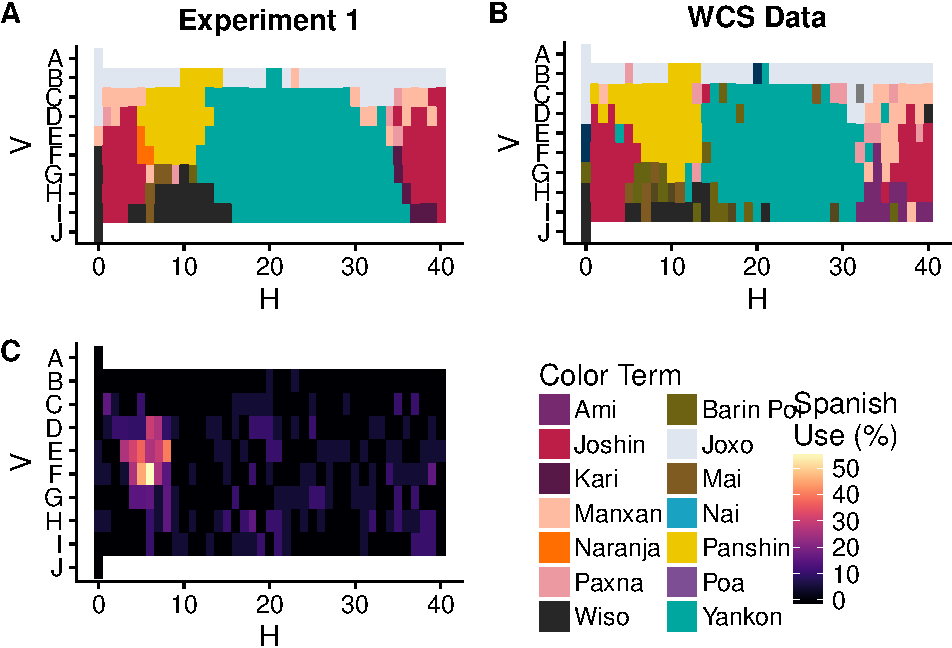
\includegraphics{amazon_color_files/figure-latex/adultfigure-1.pdf}
\caption{\label{fig:adultfigure}(A and B) Plots of the modal term given for
a particular chip. Color coordinates were represented in 2-D Munsell
space. Modal responses were given by SK adults during (A) the original
World Color Survey and during (B) our Experiment 1. (C) Heat map of
prevalence of Spanish-language responses during Experiment 1. Legends
for all three subplots located in the bottom-right quadrant.}
\end{figure}

Broadly speaking, our results were quite similar to the WCS findings.
Figure 1 shows a comparison between our data (Panel A) and the WCS
(panel B). The basic level colors in our data were quite similar, as
well. All participants described at least 1 chip with the following set
of color terms: light/white (\enquote{joxo}), dark/black
(\enquote{wiso}), yellow (\enquote{panshin}), red (\enquote{joshin}),
and green/blue (\enquote{yankon}). Most (79\%) participants also used
described at least 1 chip as faded or \enquote{manxan}, referring to a
chip's saturation. In terms of overall popularity, participants on
average described 32\% of chips as \enquote{yankon} (\emph{SD} = 10\%)
followed by \enquote{joshin} (\emph{M} = 12\%, \emph{SD} = 6\%),
\enquote{joxo} (10\%, 5\%), \enquote{panshin} (9\%, 4\%),
\enquote{manxan} (7\%, 7\%), and \enquote{wiso} (6\%, 4\%).

One departure from the Berlin-Kay data was that 59\% of adults described
at least 1 chip using a Spanish-language color term, accounting for 4\%
of all responses (Figure 1, Panel C). In particular, Spanish use reached
as high as 55\% when participants were asked to label chips that English
speakers would consider to be orange. However, there was a high amount
of variability in Spanish use between subjects (\emph{M} = 4\%,
\emph{SD} = 12\%) which neither participant age (\emph{p} = 0.87) nor
reported age of Spanish introduction (\emph{p} = 0.56) failed to
predict. Some subjects never responding in Spanish whereas one
participant responded in Spanish for 71\% of all trials despite all
sessions being conducted entirely in the Shipibo-Konibo language. While
we can only speculate as to this participant's motivations, it seems
likely that they were more familiar with the Spanish vocabulary or
viewed it as more precise.

Participants on average described 69\% of chips using a SK basic color
term like \enquote{yankon} (\emph{SD} = 22\%). Some participants
described chips using SK ad-hoc color terms, such as \enquote{nai} or
\emph{sky} for blue chips (\emph{M} = 11\%, \emph{SD} = 12\%), or ad hoc
terms referring to saturation or luminosity of a chip, such as
\enquote{manxan} (\emph{M} = 7\%, \emph{SD} = 7\%). Virtually all
instances where a participant responded in Spanish involved a Spanish
basic color term such as \enquote{rojo} (\emph{M} = 4\%, \emph{SD} =
10\%). In other words, participants typically only responded in Spanish
to label chips into basic categories; they relied on Shipibo-Konibo for
other descriptors.

Given these data, we next moved on to exploring the development of SK
color vocabulary in childhood. Experiment 2 tests production and
comprehension of SK color terms using SK-prototypical color chips;
Experiment 3 tests children in Spanish using Spanish-prototypical chips.

\section{Experiment 2}\label{experiment-2}

In Experiment 2, we tested children on their production and
comprehension skills with a set of chips representing the prototypical
colors for common SK color terms.

\subsection{Methods}\label{methods-1}

\subsubsection{Participants}\label{participants-1}

\begin{table}[tbp]
\begin{center}
\begin{threeparttable}
\caption{\label{tab:unnamed-chunk-2}Demographics of participants in Experiment 2.}
\begin{tabular}{lll}
\toprule
Age Group & \multicolumn{1}{c}{N} & \multicolumn{1}{c}{Male}\\
\midrule
5 & 3 (5\%) & 1 (33\%)\\
6 & 8 (14\%) & 3 (38\%)\\
7 & 12 (21\%) & 4 (33\%)\\
8 & 15 (26\%) & 5 (33\%)\\
9 & 10 (18\%) & 5 (50\%)\\
10 & 4 (7\%) & 2 (50\%)\\
11 & 5 (9\%) & 3 (60\%)\\
\bottomrule
\end{tabular}
\end{threeparttable}
\end{center}
\end{table}

The Pontificia Universidad Católica del Perú's Institutional Review
Board approved our study protocol. We recruited 57 5- to 11-year-old
children (23 boys). Table 1 shows the distribution of ages and genders.
Fifteen children were recruited from neighborhoods in Yarinacocha, in
the Pucallpa region of Peru, as well as in 42 children from Bawanisho, a
native community settled along the Ucayali River, south of Pucallpa.
Children were recruited either through their parents or through local
schools. When recruited at school, consent for participation was
collected from both the teachers and the parents; otherwise, only
consent from the parents was collected.

\subsubsection{Materials}\label{materials-1}

Based on findings of Experiment 1, we selected out 8 color chips that
were prototypical instances of prominent SK color terms. These color
chips were blue (WCS n°1), green (WCS n°234), red (WCS n°245), white
(WCS n°274), yellow (WCS n°297), black (WCS n°312), greeny-yellow (WCS
n°320), and purple (WCS n°325). These color chips were exactly the same
as those used in Experiment 1; the only difference was that adult
participants in Study 1 were presented with these chips along the rest
of their assigned 165 chip set. Child participants only had these 8
chips.

\subsubsection{Procedure}\label{procedure-1}

The production and comprehension tasks were both conducted in SK. In
both tasks, children were seated in front of the experimenter. A table
on which the color chips were display stood between them. The production
task was always performed before the comprehension task.

\textbf{Production task.} The procedure was very similar to that of
Experiment 1. Children were first introduced to the whole procedure and
the general goal of the study. It was specified that they would be
expected to provide color terms in SK (and not in Spanish). Children
were then asked: \enquote{What is the color of this chip?}. As with
adults, we used follow-up questions to elicit basic color terms when the
terms children initially provided were not basic. When children provided
Spanish color terms, the experimenter would write down their response
but further ask: \enquote{What is the name of this color in SK?} When
children replied \enquote{I don't know} to this prompt, the experimenter
would not ask further questions and would move forward to the next color
chip. As a result, responses of some children include only non-basic SK
color terms or Spanish color terms. In total, we collected production
data for 8 color chips. For each chip, the data include either one
response (when children provided a SK basic color term in the first
trial) or two or three responses (when children's initial responses were
either non-basic and/or in Spanish).

Further, Experiment 1 showed that for some of these color terms, only
one response was accurate, while for others, several responses were
equally correct. For example, responses during Experiment 1 to a
particular purple chip ranged from red to blue with some using the terms
ami (\enquote{flower}) or pua (\enquote{yam}) as common descriptors.
Accuracy was coded based on the results derived from Experiment 1: if at
least 15\% of participants in Experiment 1 labeled a chip with a
particular term, we considered a trial to be correct if the child made
the same pairing, regardless of whether the term as a basic or ad-hoc
color term.

\textbf{Comprehension task.} The 8 color chips of the production task
were simultaneously displayed in front of the children. The experimenter
would then ask: \enquote{Can you give me the {[}color{]} chip?} In
total, the comprehension of 9 SK color terms was tested. The choice of
these terms was based on the findings of Experiment 1. Not all of them
were basic, but all of them stood out as being prominent in the SK color
system. The 9 terms used as prompts included: yankon
(\enquote{green/blue}), joshin (\enquote{red}), panshin
(\enquote{yellow}), joxo (\enquote{white), wiso (}black\enquote{), nai
(}blue\enquote{), and barin poi (}greeny-yellow\enquote{). In addition,
as Experiment 1 revealed that two non-basic terms are widely used to
refer to green and purple, two words were used to test comprehension of
each of these two colors: pei/xo (}green\enquote{) and ami/pua
(}purple``).

When the experimenter asked children to pick up a color that was
instantiated by several chips, we followed the following procedure. The
experimenter would ask: \enquote{Can you give me the {[}color{]} chip?}
Children would then pick up a chip. The response would be registered and
the chip be taken out of the table. As a result, only 7 chips would be
remaining on the table. The experimenter would subsequently ask:
\enquote{Can you give me another {[}color{]} chip?}. Children would then
pick up a new chip. The response would be registered and the chip be
taken out of the table. The experimenter would then ask the same
question again until a total of as many times as there were correct
instances. Thus, for example, for yankon four chips would be elicited,
while for joshin, two chips would be elicited. Like the preceding
production task, accuracy was scored based on responses given in Study
1. If a child chose a particular chip, their choice was deemed accurate
if at least 15\% of participants during Study 1 made the same chip-label
pairing.

\subsection{Results and Discussion}\label{results-and-discussion-1}

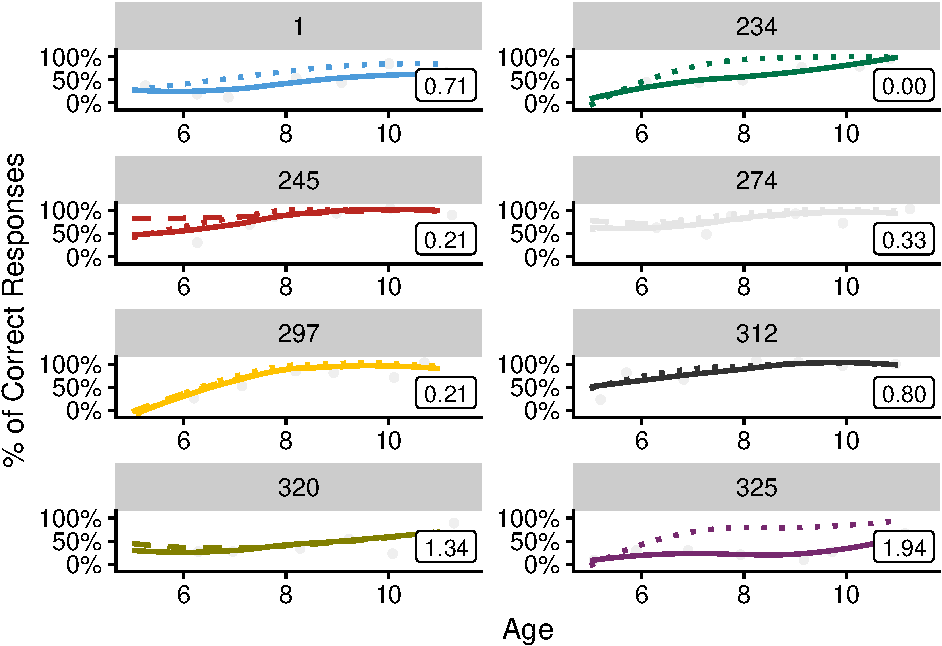
\includegraphics{amazon_color_files/figure-latex/childfigure-1.pdf}
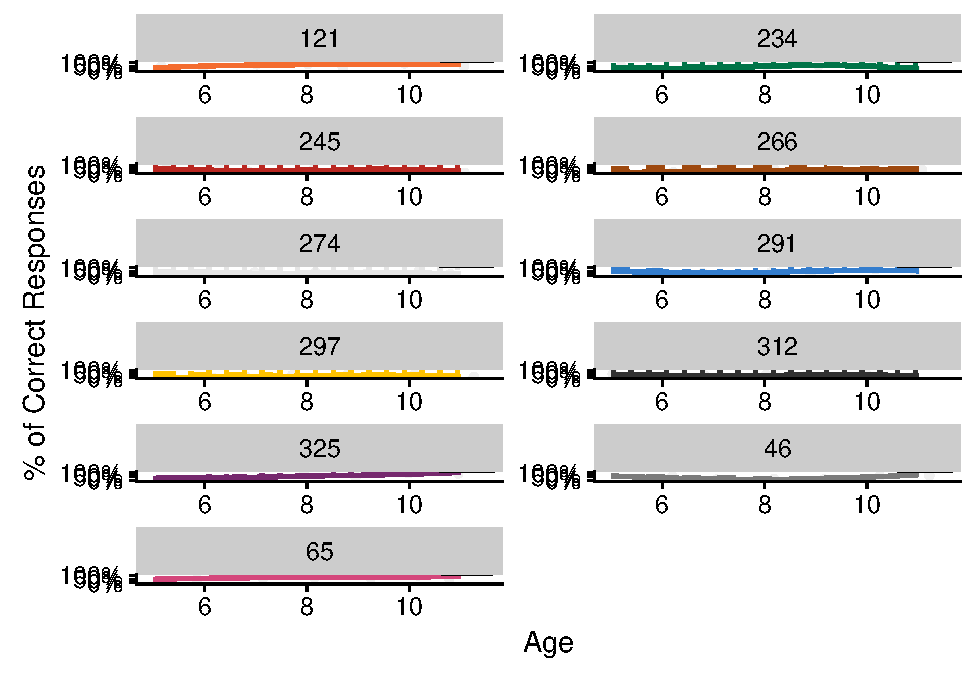
\includegraphics{amazon_color_files/figure-latex/childfigure-2.pdf}

\textbf{Production.} Children's production accuracy increased
substantially across nearly all color chips in the age range that we
tested. Figure 2, left panels shows the accuracy of children's first
production, both in SK (solid line) and in either language (dashed
line). To quantify these developmental trends, we fit two generalized
linear mixed effects models, one for the accuracy of SK production and
one for the accuracy of production in either language. Both of these
predicted accuracy as a function of the child's age, and included random
intercepts for color chip and for participant, as well as a random slope
of age by color chip. Age was a significant predictor in both models:
\(\beta = 1.05\), SE = 0.28, \(p = 0\) and \(\beta = 1.11\), SE = 0.23,
\(p < .0001\).

Over a quarter (28\%) of all responses were given in Spanish, and the
distribution of Spanish responses was non-random. Children tended to
respond in Spanish when presented with a chip with low naming consensus
among adult participants in Experiment. We computed the naming entropy
for each chip by computing the probabilities for each chip \(c\) to be
named with a particular label \(l\) (\(p(l \mid c)\)) and then taking
\(H(c) = - \sum{p(l\mid c) \log[p(l \mid c)]}\) (see inset entropy
values by chip in Figure 2).

To assess the hypothesis that naming entropy in adults was related to
Spanish use in children, we fit a mixed effects model predicting Spanish
responses as a function of age, entropy of the chip's naming
distribution for adults, and their interaction. We included random
intercepts for color chip and for participant, but our model did not
converge with a random slope term and so we pruned this term following
our lab's standard operating procedure. We found a reliable effect of
entropy (\(\beta = -6.09\), SE = 2.38, \(p = 0.01\)) and an interaction
between age and entropy (\(\beta = -3.97\), SE = 1.49, \(p = 0.01\)),
suggesting that adults' uncertainty regarding naming was related to
children's likelihood of producing Spanish labels.

Another possible reason to use Spanish would be if children fail to
recall the proper SK color term but do know the proper mapping in the
Spanish. They may also choose to respond with a same-language but
adjacent color term )such as \enquote{joshin} for a
\emph{panshin}-colored chip). In our next analysis, we aggregate across
chips and examine the pattern of responses, categorizing them as
same-language, adjacent, and different-language.

Using a mixed-effects model, we found a significant improvement in
accuracy scores when we allowed different-language but corresponding
responses (\emph{p} \textless{} 0.001) but no significant change when
allowing for same-language but adjacent responses (\emph{p} = 0.454).

\begin{verbatim}
## # weights:  30 (20 variable)
## initial  value 236.587373 
## iter  10 value 120.155378
## iter  20 value 113.858407
## iter  30 value 113.838510
## iter  40 value 113.836190
## final  value 113.836165 
## converged
\end{verbatim}

\begin{verbatim}
## # weights:  10 (4 variable)
## initial  value 236.587373 
## iter  10 value 119.446075
## final  value 119.333166 
## converged
## # weights:  15 (8 variable)
## initial  value 236.587373 
## iter  10 value 121.753001
## final  value 118.436067 
## converged
\end{verbatim}

\textbf{Comprehension.}

\section{Experiment 3}\label{experiment-3}

Noting the level of bilingualism in Experiment 2, we designed Experient
3 as its complement. In Experiment 3, we tested children entirely in
Spanish with a set of chips representing prototypical colors for the
Spanish color system.

\begin{table}[tbp]
\begin{center}
\begin{threeparttable}
\caption{\label{tab:unnamed-chunk-4}}
\begin{tabular}{llll}
\toprule
Age Group & \multicolumn{1}{c}{Age (SD)} & \multicolumn{1}{c}{N} & \multicolumn{1}{c}{Male}\\
\midrule
5-years-old & 5.2 (0.35) & 2 (4\%) & 1 (50\%)\\
6-years-old & 6.2 (0.21) & 2 (4\%) & 0 (0\%)\\
7-years-old & 7.3 (0.33) & 11 (24\%) & 4 (36\%)\\
8-years-old & 8.4 (0.3) & 9 (20\%) & 1 (11\%)\\
9-years-old & 9.4 (0.27) & 11 (24\%) & 4 (36\%)\\
10-years-old & 10.3 (0.35) & 8 (17\%) & 3 (38\%)\\
11-years-old & 11.2 (0.32) & 3 (7\%) & 3 (100\%)\\
\bottomrule
\end{tabular}
\end{threeparttable}
\end{center}
\end{table}

\subsubsection{Participants}\label{participants-2}

Our protocol received ethical approval from Pontificia Universidad
Católica del Perú's Institutional Review Board. Children were recruited
in a SK neighborhood of Yarinacocha (Bena Jema) as well as in Bawanisho.
As before, children were recruited either through their parents or
through the local school. When recruited at school, consent for
participation was collected from both the teachers and the parents;
otherwise, only consent from the parents was collected. Data were
collected from a total of 46 children (16 boys) who were between the
ages of 5 and 11 years old.

\subsubsection{Materials}\label{materials-2}

Even though participants of Experiment 1 were instructed to give color
terms in SK, some Spanish color terms were provided (this was especially
true of young adult participants). Based on these data and on previous
studies of Spanish color systems, we singled out 11 color chips that
were prototypical instances of prominent Peruvian Spanish color terms.
These color chips were grey (WCS n°46), pink (WCS n°65), orange (WCS
n°121), green (WCS n°234), red (WCS n°245), brown (WCS n°266), white
(WCS n°274), blue (WCS n°291), yellow (WCS n°297), black (WCS n°312) and
purple (WCS n°325). (To visualize the hue of these chips, see Appendix
1.) These color chips were exactly the same as those used in Experiment
1; the only difference was that while 330 chips were used in Experiment
1, only 11 of them were used in Experiment 3. It is worth noting that
six chips were shared between Experiment 2 and Experiment 3.

\subsubsection{Procedure}\label{procedure-2}

Since SK children are not very fluent in Spanish, the production and
comprehension tasks were both conducted in SK, and Spanish was only used
for color terms (i.e., Spanish color terms were embedded in SK
sentences). In both tasks, children were seating in front of the
experimenter; a table (on which the color chips were displayed) was
standing between them. As in Experiment 2, the production task was
always performed before the comprehension task.

Production task. The procedure was the same as that of Experiment 2.
Children were first introduced to the whole procedure and the general
goal of the study. It was specified that they would be expected to
provide color terms in Spanish (and not in SK). Children were then
asked: \enquote{what is the color of this chip?}. When children provided
SK color terms, the experimenter would write down their response but
further ask: \enquote{what is the name of this color in Spanish?}. When
children were replying \enquote{I don't know} to this prompt, the
experimenter would not ask further questions and would move forward to
the next color chip. As a result, responses of some children include
only non-basic Spanish color terms or SK color terms. In total, we
collected production data for 11 color chips. For each chip, the data
include either one response (when children provided a Spanish basic
color term in the first trial) or two or three responses (when
children's initial responses were either non-basic and/or in SK).

Comprehension task. The procedure was similar to that of the
comprehension task of Experiment 2. The 11 color chips of the production
task were simultaneously displayed in front of the children. The
experimenter would then ask: \enquote{Can you give me the \_\_\_ chip?}
(where ``\_\_\_" stands for a color term). In total, the comprehension
of 11 Spanish color terms was tested.

The choice of these terms was based on previous studies examining
Spanish color terms as well as on Experiment 1 (as we have seen, SK
adults sometimes resorted to Spanish color terms to name the color
chips). The 11 terms used as prompts included: blanco (\enquote{white}),
verde (\enquote{green}), rojo (\enquote{red}), amarillo
(\enquote{yellow}), azul (\enquote{blue}), negro (\enquote{black}),
naranja (\enquote{orange}), gris (\enquote{grey}), morado
(\enquote{purple}), marrón (\enquote{brown}), and rosa (\enquote{pink}).
Since each color term was instantiated by only one color chip, no term
required the special procedure that was followed in Experiment 2 for
yankon, joshin and pei/xo.

\subsection{Results and Discussion.}\label{results-and-discussion.}

\textbf{Production} Unlike Study 2, age did not have a significant
relationship with children's production accuracy. The right panels on
Figure 2 show the accuracy of children's first production, both in SK
(solid line), in either language (dashed line), or including adjacent
color terms (dotted line). To quantify these developmental trends, we
fit two generalized linear mixed effects models, one for the accuracy of
SK production and one for the accuracy of production in either language.
Both of these predicted accuracy as a function of the child's age, and
included random intercepts for color chip and for participant, as well
as a random slope of age by color chip. Age failed to gain significance
as a predictor in either models: \(\beta = 0.32\), SE = 0.20,
\(p = 0.11\) and \(\beta = 0.43\), SE = 0.16, \(p < .0001\).

Similar to Experiment 2, over a quarter of all responses (\emph{M} =
28\%, \emph{SD} = 18\%) were given in another language (Shipibo in this
case). There was significant variation in language-switching with some
children completing the entire task in Spanish while others responded to
upwards of 59\% of trials in Shipibo. Similar to Experiment 2, there was
no significant correlation between age and label accuracy (\emph{p} =
0.063) or between age and language-switching (\emph{p} = 0.908). Still,
we found that participants tended to respond in Shipibo when presented
with items that had low entropy among SK adults during Experiment 1 (p =
0.006). This suggests that participants across Studies 2 and 3 preferred
to respond in Shipibo when presented with a high-consensus chip and in
Spanish when shown a low-consensus chip.

\textbf{Overextensions.}

Similar to Experiment 2, we adopted alternative scoring to accommodate
language-switching from Spanish to Shipibo-Konibo and same-language
adjacent responses. Using a mixed-effects model, we did not find that
age explained a significant amount of the variation seen in accuracy
(\emph{p} = 0.124), in concordance with earlier analyses. However, we
did find that participants made use of both mapping strategies of either
providing different-language but corresponding responses (\emph{p}
\textless{} 0.001) or same-language but adjacent responses (\emph{p} =
0.002). Between Studies 2 and 3, we find frequent use of language
switching but only Experiment 3 shows significant use of same-language
but adjacent terms as well. This discrepancy, along with the lack of an
age correlation, can be due to foreign language exposure. Children may
be exposed to Spanish at a young age but do not receive any formal
Spanish education until later in adolescence. With a limited knowledge
of Spanish color terms, children may spontaneously provide Spanish color
terms during the Shipibo-language Experiment 2 but may struggle to
succeed during Spanish-language Experiment 3. This suggests that
children may rely on either strategy to communicate a color label to the
best of their knowledge set.

\begin{verbatim}
## # weights:  30 (20 variable)
## initial  value 202.789177 
## iter  10 value 72.998387
## iter  20 value 72.094921
## iter  30 value 72.071216
## iter  40 value 72.069217
## final  value 72.069182 
## converged
\end{verbatim}

\begin{verbatim}
## # weights:  10 (4 variable)
## initial  value 202.789177 
## iter  10 value 82.649326
## final  value 82.642259 
## converged
\end{verbatim}

\textbf{Comparisons between Studies 2 \& 3. - Unfinished plots}

\begin{figure}
\centering
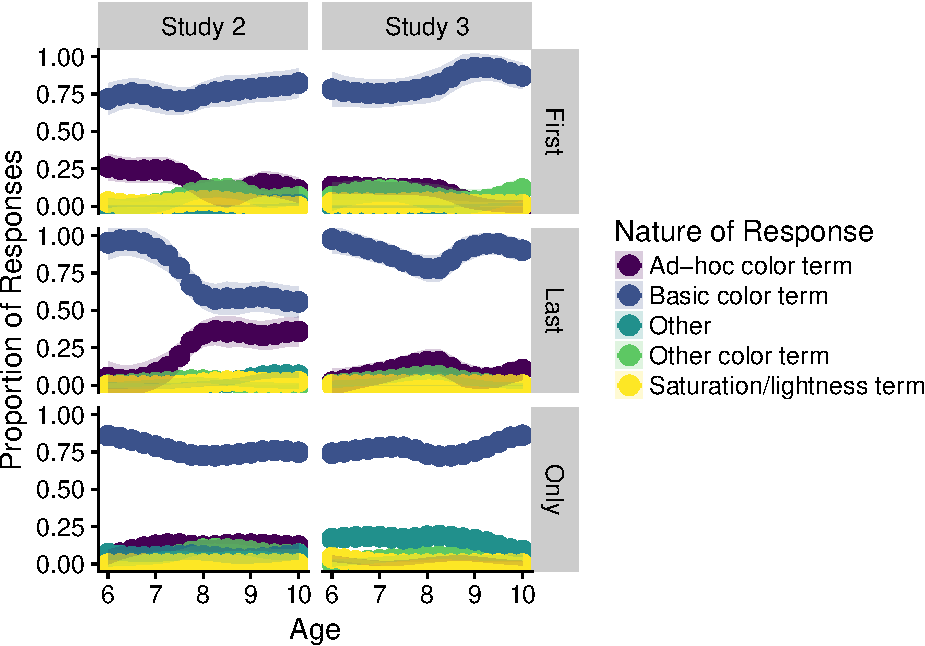
\includegraphics{amazon_color_files/figure-latex/crossstudy_accuracystrats-1.pdf}
\caption{}
\end{figure}

\section{General Discussion}\label{general-discussion}

TO BE PASTED FROM GOOGLE DOC

\newpage

\section{References}\label{references}

\begingroup
\setlength{\parindent}{-0.5in} \setlength{\leftskip}{0.5in}

\hypertarget{refs}{}
\hypertarget{ref-berlin2009}{}
Kay, P., Berlin, B., Maffin, L., Merrifield, W. R., \& Cook, R. (2009).
\emph{The world color survey}. Stanford, CA: Center for the Study of
Language; Information.

\endgroup






\end{document}
